\documentclass[presentation, 12pt, aspectratio=169, t]{beamer}
\usepackage[T1]{fontenc}
\usepackage[utf8]{inputenc}
\usepackage[british]{babel}
\usepackage{bm, braket, tikz, textpos, amsmath, amssymb, transparent, mathtools, xcolor}
\usepackage{minted}
\usepackage{plex-mono, mathpazo}
\usepackage{plex-serif, plex-sans}
\usepackage[export]{adjustbox}
\usepackage[numbers,sort&compress]{natbib}
\usepackage{doi,hyperref}

\definecolor{solbase03}{HTML}{002b36}
\definecolor{solbase02}{HTML}{073642}
\definecolor{solbase01}{HTML}{586e75}
\definecolor{solbase00}{HTML}{657b83}
\definecolor{solbase0}{HTML}{839496}
\definecolor{solbase1}{HTML}{93a1a1}
\definecolor{solbase2}{HTML}{eee8d5}
\definecolor{solbase3}{HTML}{fdf6e3}
\definecolor{solyellow}{HTML}{b58900}
\definecolor{solorange}{HTML}{cb4b16}
\definecolor{solred}{HTML}{dc322f}
\definecolor{solmagenta}{HTML}{d33682}
\definecolor{solviolet}{HTML}{6c71c4}
\definecolor{solblue}{HTML}{268bd2}
\definecolor{solcyan}{HTML}{2aa198}
\definecolor{solgreen}{HTML}{859900}

\definecolor{purple-60}{HTML}{8a3ffc}
\definecolor{magenta-40}{HTML}{ff7eb6}
\definecolor{magenta-60}{HTML}{d02470}

\hypersetup{colorlinks=true, linkcolor=solbase03, urlcolor=purple-60}

\makeatletter
\newcommand*\providelength[1]{\@ifundefined{\expandafter\@gobble\string#1}{\newlength{#1}}{}}

\newcommand*\ferris{{\smash{\raisebox{-0.4ex}{\includegraphics[height=2ex]{ferris}}}}}
\newcommand*\cicon{{\smash{\raisebox{-0.4ex}{\includegraphics[height=2ex]{c}}}}}
\newcommand*\pyicon{{\smash{\raisebox{-0.4ex}{\includegraphics[height=2ex]{python}}}}}

\newcommand*\supplementbegin{%
    \newcounter{lastframenumber}%
    \setcounter{lastframenumber}{\value{framenumber}}%
    \let\old@insertframenumber\insertframenumber%
    \let\old@inserttotalframenumber\inserttotalframenumber%
    \renewcommand\insertframenumber\textellipsis%
    \renewcommand\inserttotalframenumber\textellipsis}
\newcommand*\supplementend{%
    \setcounter{framenumber}{\value{lastframenumber}}%
    \renewcommand\insertframenumber\old@insertframenumber%
    \renewcommand\inserttotalframenumber\old@inserttotalframenumber}
\makeatother

\usetheme{Boadilla}

\makeatletter
\def\beamer@tsfont{\sffamily}
\def\beamer@sfont{\sffamily}
\def\familydefault{\sfdefault}
\def\mathfamilydefault{\rmdefault}
\setbeamerfont{title}{family=\rmfamily}
\setbeamerfont{frametitle}{family=\rmfamily}
\setbeamerfont{tiny structure}{family=\beamer@tsfont}
\setbeamerfont{structure}{family=\beamer@sfont}
\makeatother

\setbeamertemplate{navigation symbols}{}

\setbeamertemplate{itemize items}[circle]
\setbeamercolor{itemize item}{fg=purple-60}
\setbeamercolor{itemize subitem}{fg=purple-60}
\setbeamertemplate{enumerate items}[default]
\setbeamercolor{enumerate item}{fg=purple-60}
\setbeamercolor{description item}{fg=purple-60}
\setlength{\leftmargini}{2ex}
\setlength{\leftmarginii}{2.2ex}

%\setbeamercolor{normal text}{fg=black,bg=solbase3}
\setbeamercolor{alerted text}{fg=solred}
\setbeamercolor{titlelike}{fg=magenta-60}

\definecolor{solbase2a}{RGB}{232, 223, 205}
\definecolor{solbase2b}{RGB}{223, 214, 196}
\definecolor{solbase2c}{RGB}{215, 206, 188}
\setbeamercolor{author in head/foot}{fg=solbase03, bg=solbase2c}
\setbeamercolor{title in head/foot}{fg=solbase03, bg=solbase2b}
\setbeamercolor{date in head/foot}{fg=solbase03, bg=solbase2a}

\setbeamertemplate{blocks}[rounded][shadow=false]
\addtobeamertemplate{block begin}{}{\vspace*{1.2\smallskipamount}\centering}
\addtobeamertemplate{block end}{\vspace*{\smallskipamount}}{}
\addtobeamertemplate{block alerted begin}{}{\centering}
\addtobeamertemplate{block example begin}{}{\centering}
\setbeamerfont{block title}{size=\footnotesize}
\setbeamercolor{block title}{fg=black,bg=solbase2}
\setbeamercolor{block body}{bg=solbase3}


\setbeamercovered{transparent=0}

\setbeamersize{text margin left=0.08\paperwidth}
\setbeamersize{text margin right=0.08\paperwidth}

\usetikzlibrary{calc, arrows.meta, positioning, decorations.pathreplacing, external}

\usemintedstyle{solarized-light}

\pdfstringdefDisableCommands{%
    \def\underline#1{#1}%
    \def\\{}
    \def\url#1{}
}

\setbeamerfont{title}{size=\large}  % This particular title is just a little too big for `\Large`.
\title{Moving a quantum compiler from Python to Rust}
\author[Jake Lishman]{Jake Lishman\\\url{jake.lishman@ibm.com}}
\institute{IBM}
\date{16th of October, 2026}
\begin{document}


\begin{frame}
\titlepage
\end{frame}

\begin{frame}\frametitle{About me}
\begin{itemize}\itemsep=0.8\baselineskip
\item Work for IBM Research
\item Background in physics of quantum computing with trapped ions
\item Technical lead of\ \raisebox{-0.15em}{
\includegraphics[width=1em]{qiskit-icon-purple-60}}\,Qiskit, a quantum compiler
\end{itemize}
\bigskip
{\centering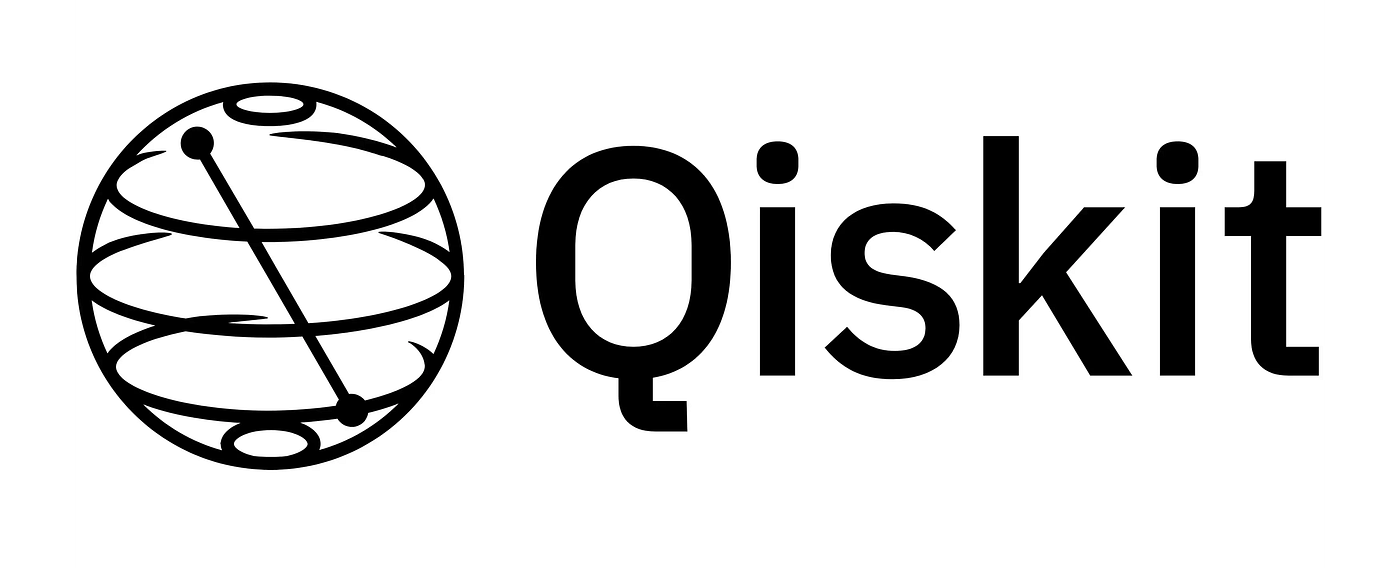
\includegraphics[width=0.3\textwidth]{qiskit-light}\par\url{https://github.com/Qiskit/qiskit}\par}
\end{frame}

\begin{frame}\frametitle{What is a quantum compiler anyway?}
\pause
\begin{block}<+->{}
Depends on who you ask!
\end{block}
\bigskip
\begin{onlyenv}<+->\begin{itemize}\itemsep=0.8\baselineskip
\item We'll talk about an early `gate-model' quantum virtual machine.
\item No `regular' machine code for control hardware to generate.
\item No control flow.
\item Input programs are already rather low level.
\item Rewrite instructions into the supported set.
\item Resolve limited connections between qubits.
\end{itemize}\end{onlyenv}
\end{frame}

\begin{frame}\frametitle{Qubits, gates and measures}
\begin{minipage}[t]{0.475\textwidth}%\vspace*{-0.6\baselineskip}%
\begin{description}[Classical]\itemsep=0.8\baselineskip
\item[Qubit] Both the `bit' and the `word' of quantum data. Also the hardware.
\item[Gate] An operation on one or more qubits.
\item[Measure] Consume one qubit into a classical bit.
\pause
\item[Classical] `Regular' computing.
\item[Circuit] A program for this virtual machine.
\end{description}
\end{minipage}\hfill\begin{minipage}[t]{0.475\textwidth}%
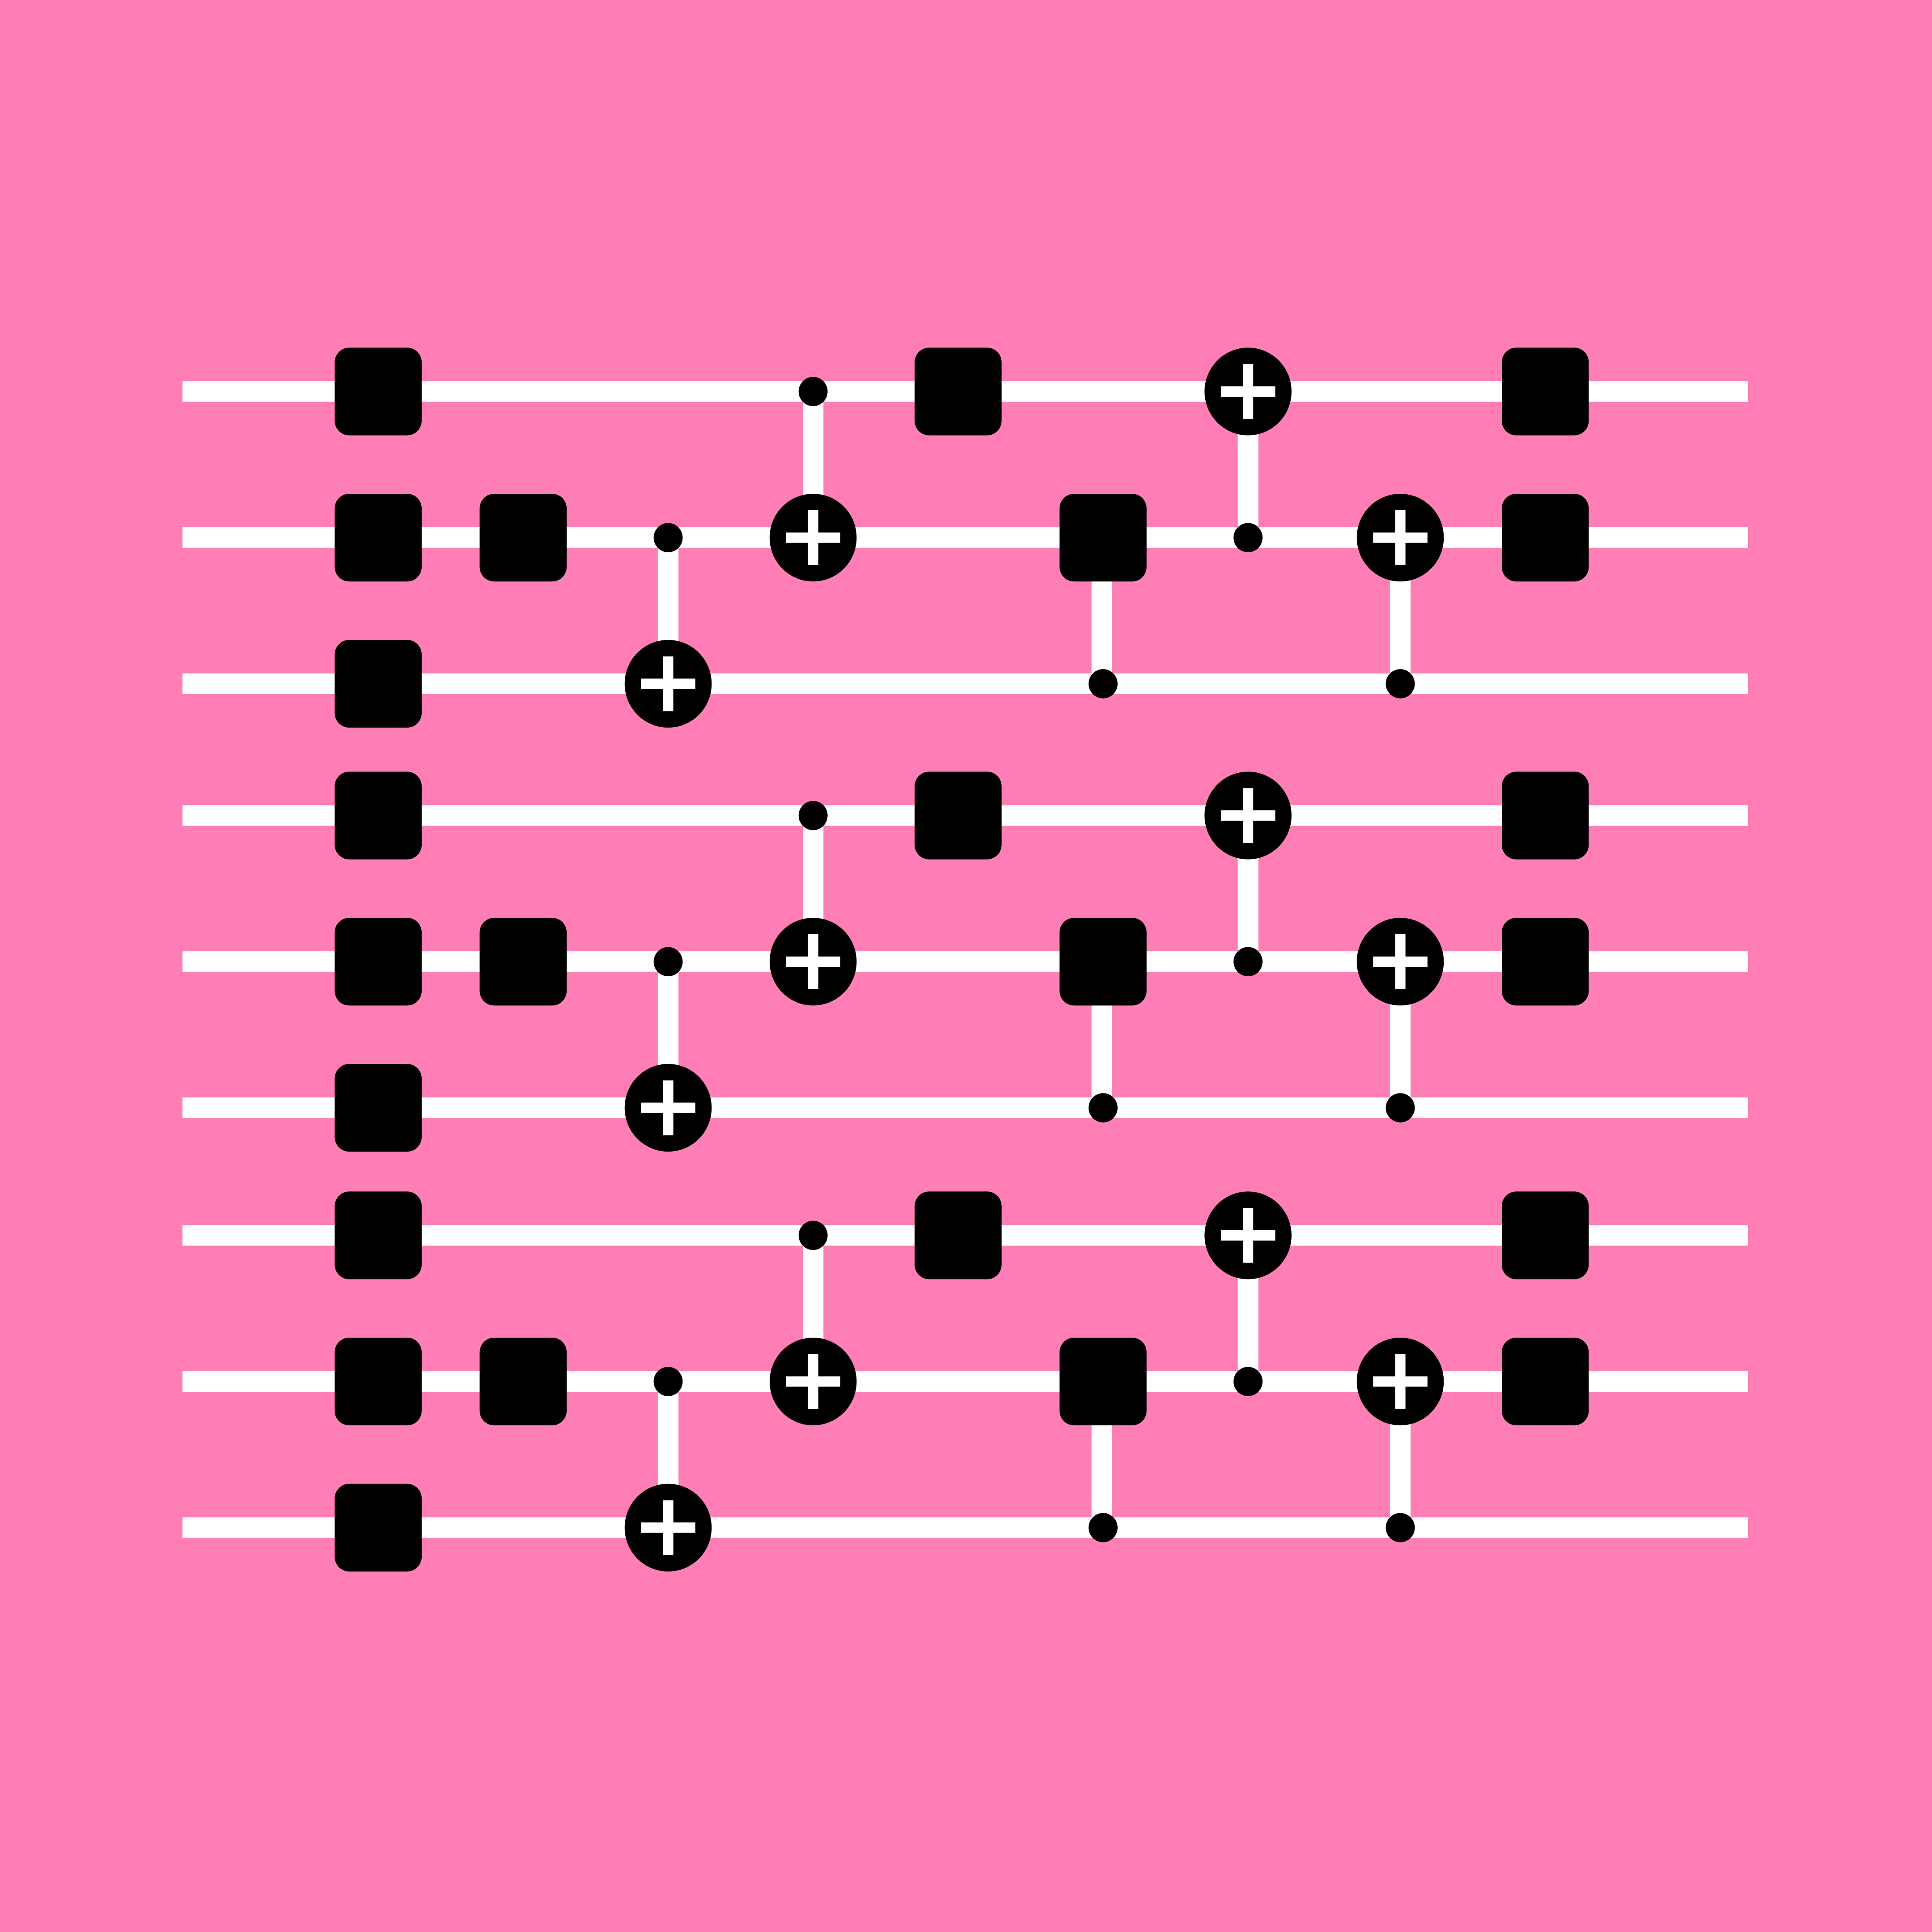
\includegraphics[valign=t, width=\textwidth]{circuit-big}%
\end{minipage}
\end{frame}

\begin{frame}\frametitle{What makes it hard?}
\begin{itemize}\itemsep=0.8\baselineskip
\item There's no such thing as a ``copy''.
\item There's no such thing as a ``store''.
\item Each qubit can only interact with its immediate neighbours.
\end{itemize}
\bigskip
{\centering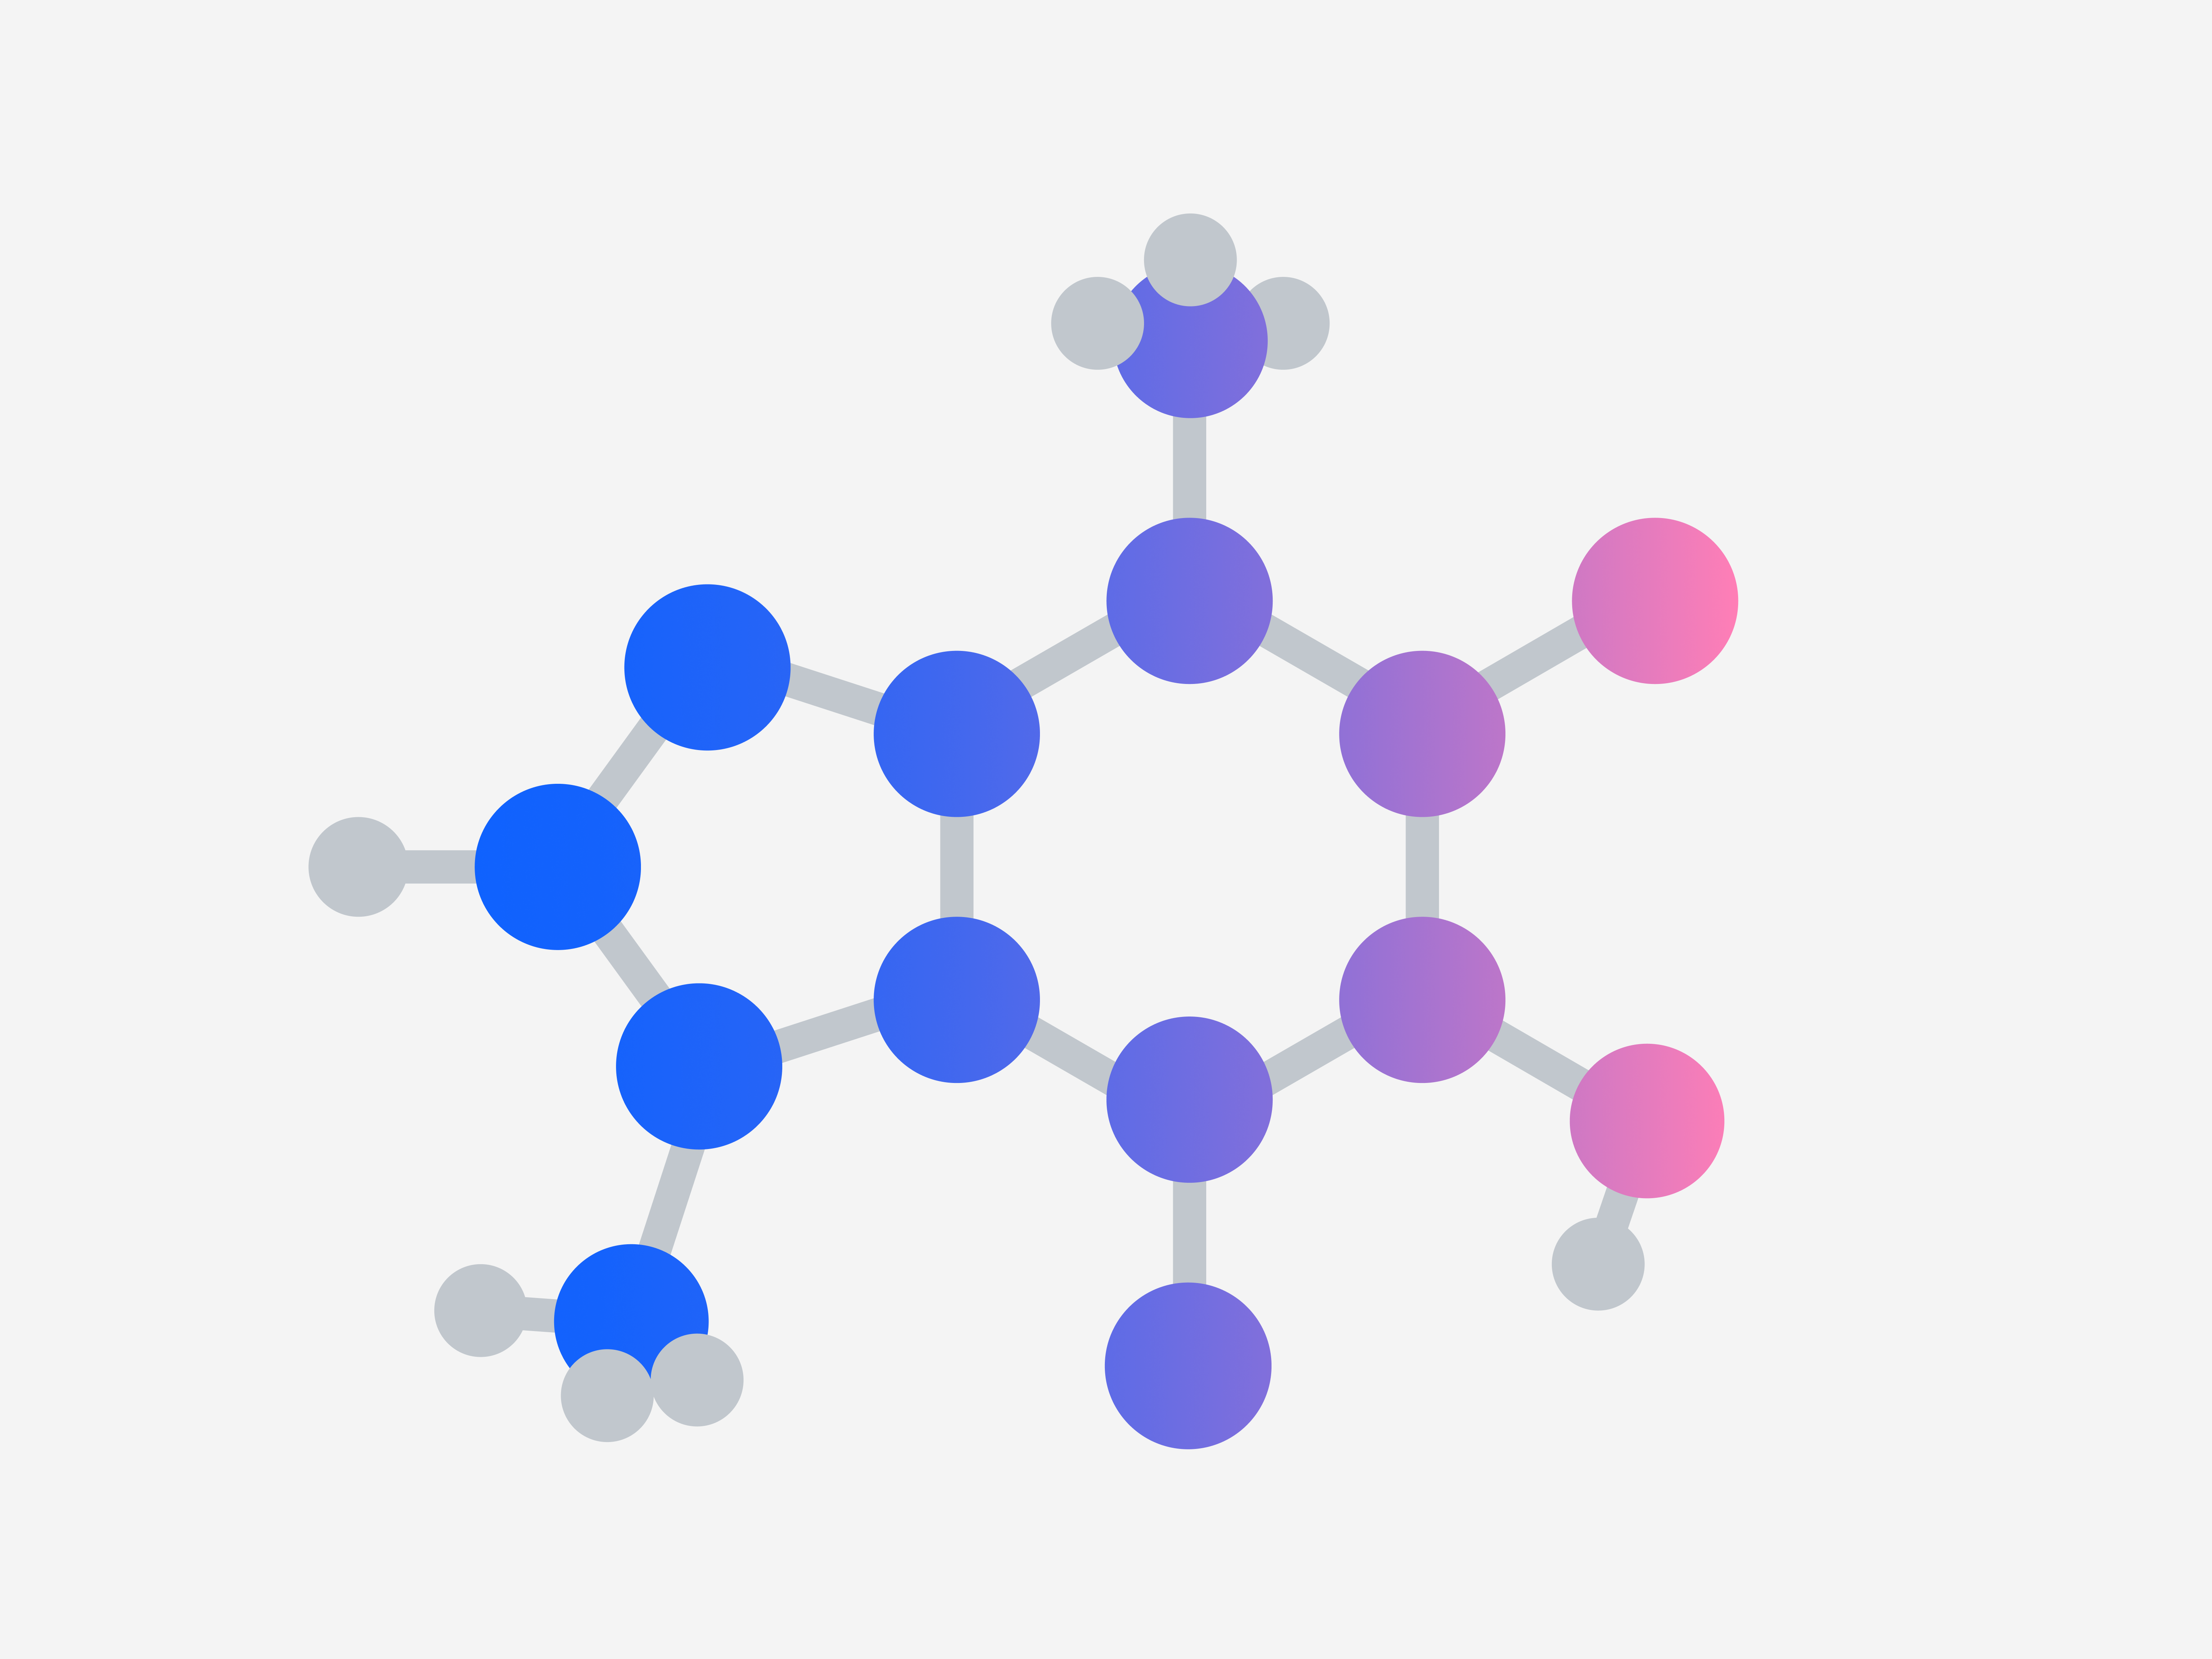
\includegraphics[width=0.4\textwidth]{not-a-qpu}\par}
\end{frame}

\begin{frame}[fragile]\frametitle{Why Python?}
\begin{minted}{python}
from qiskit import ...
import some_qpu_provider

backend = some_qpu_provider.backend("ibm_boston")
pm = generate_preset_pass_manager(2, backend)

class MyResearchPass(TransformationPass):
    def run(self, dag): ...

pm.optimization += MyResearchPass()

qc = QuantumCircuit.from_qasm_file("my_prog.qasm")
compiled = pm.run(qc)
\end{minted}
\end{frame}

\begin{frame}[fragile]\frametitle{What compilation looks like}
\begin{minipage}[t]{0.325\textwidth}\small%
\begin{minted}{openqasm3}
OPENQASM 3.0;
include
  "stdgates.inc";

qubit q[5];
bit c[5];

h q[0];
h q[2];
h q[4];
cx q[0], q[1];
cx q[0], q[2];
cx q[0], q[3];
cx q[0], q[4];
c = measure q;
\end{minted}
\end{minipage}\hfill\begin{minipage}[t]{0.3\textwidth}\scriptsize%
\pause
\begin{minted}{openqasm3}
OPENQASM 3.0;
include "stdgates.inc";
bit[5] c;
rz(pi/2) $117;
sx $117;
rz(pi) $117;
rz(-pi) $123;
sx $123;
rz(pi/2) $123;
rz(pi/2) $124;
sx $124;
rz(-pi/2) $124;
rz(pi/2) $125;
sx $125;
rz(-3*pi/2) $125;
cz $125, $124;
sx $124;
rz(pi/2) $124;
cz $124, $123;
sx $123;
\end{minted}
\end{minipage}\begin{minipage}[t]{0.25\textwidth}\scriptsize%
\begin{minted}{openqasm3}
sx $124;
cz $124, $123;
sx $123;
sx $124;
cz $124, $123;
rz(pi/2) $124;
sx $124;
rz(pi) $124;
cz $125, $126;
cz $125, $117;
sx $117;
cz $125, $124;
sx $124;
rz(pi/2) $126;
sx $126;
c[0] = measure $125;
c[1] = measure $123;
c[2] = measure $126;
c[3] = measure $117;
c[4] = measure $124;
\end{minted}
\end{minipage}
\end{frame}

\begin{frame}[fragile]\frametitle{First Rust use: a graph object}
\begin{minipage}[t]{0.475\textwidth}\small%
\begin{minted}{openqasm3}
OPENQASM 3.0;
include "stdgates.inc";

qubit q[5];
bit c[5];

h q[0];
h q[2];
h q[4];
cx q[0], q[1];
cx q[0], q[2];
cx q[0], q[3];
cx q[0], q[4];

c = measure q;
\end{minted}
\end{minipage}\hfill\begin{minipage}[t]{0.475\textwidth}
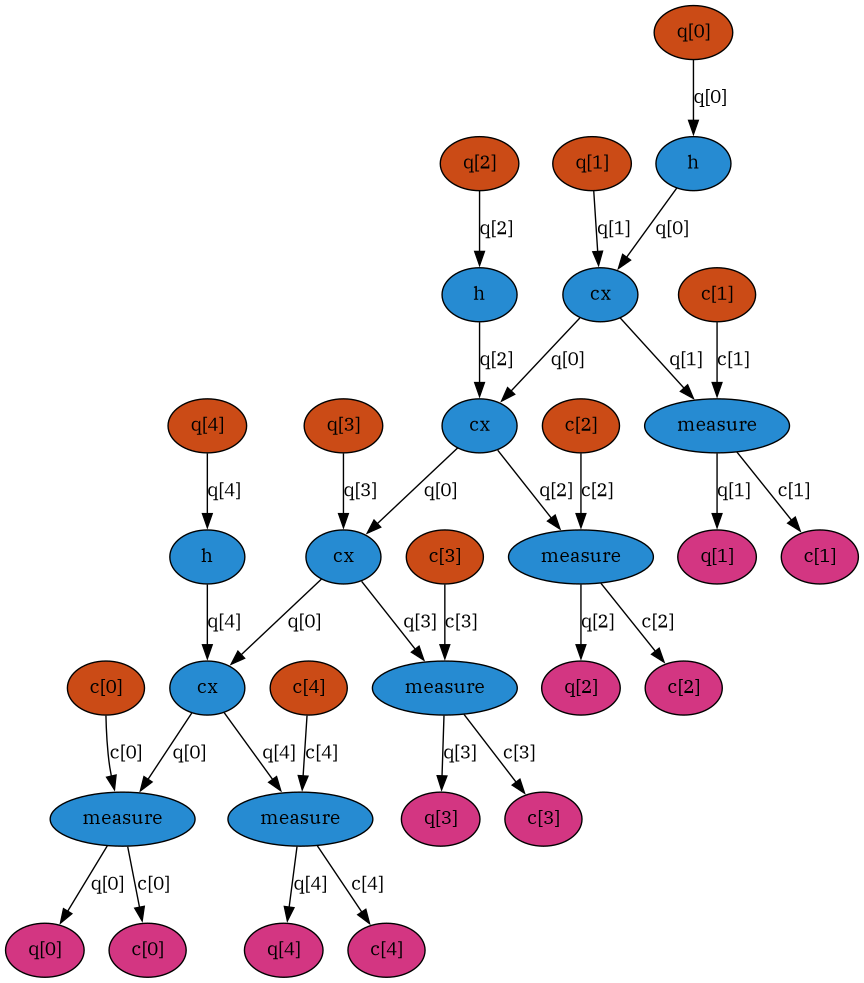
\includegraphics[valign=t, width=0.9\textwidth]{basic-dag}
\end{minipage}
\end{frame}

\begin{frame}\frametitle{Rustworkx}
\begin{block}{}
IR manipulations sped up $2\times$
\end{block}
\medskip
\begin{itemize}\itemsep=0.8\baselineskip
\item Wrapper around \texttt{petgraph}, exposed to Python with \texttt{PyO3}
\item General collection of graph algorithms and generators
\item Rust bindings in \texttt{rustworkx\_core}
\end{itemize}
\centering
\bigskip\url{https://rustworkx.org}\par
\bigskip\url{https://github.com/Qiskit/rustworkx}\par
\end{frame}

\begin{frame}\frametitle{The qubit ``routing'' problem}
\begin{minipage}[t]{0.475\textwidth}
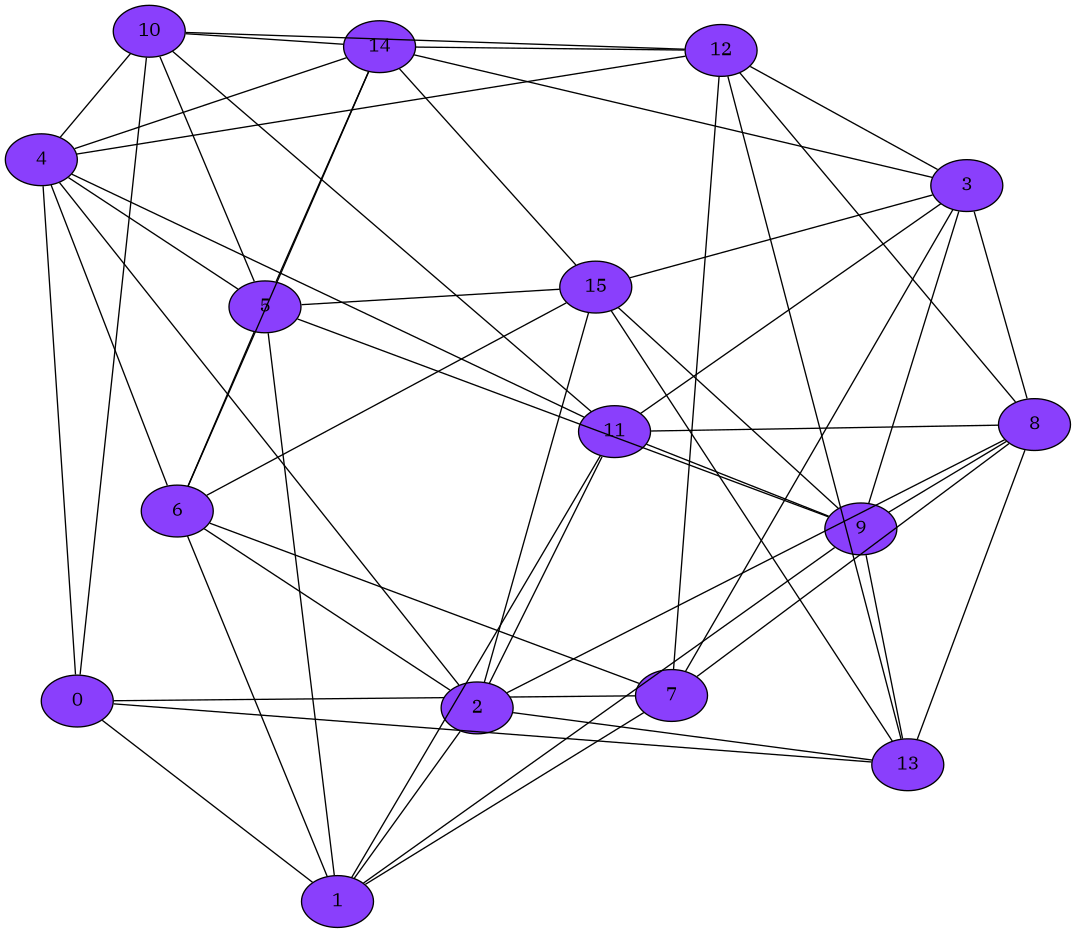
\includegraphics[valign=t, width=\textwidth]{interaction}
\end{minipage}\hfill\begin{minipage}[t]{0.475\textwidth}
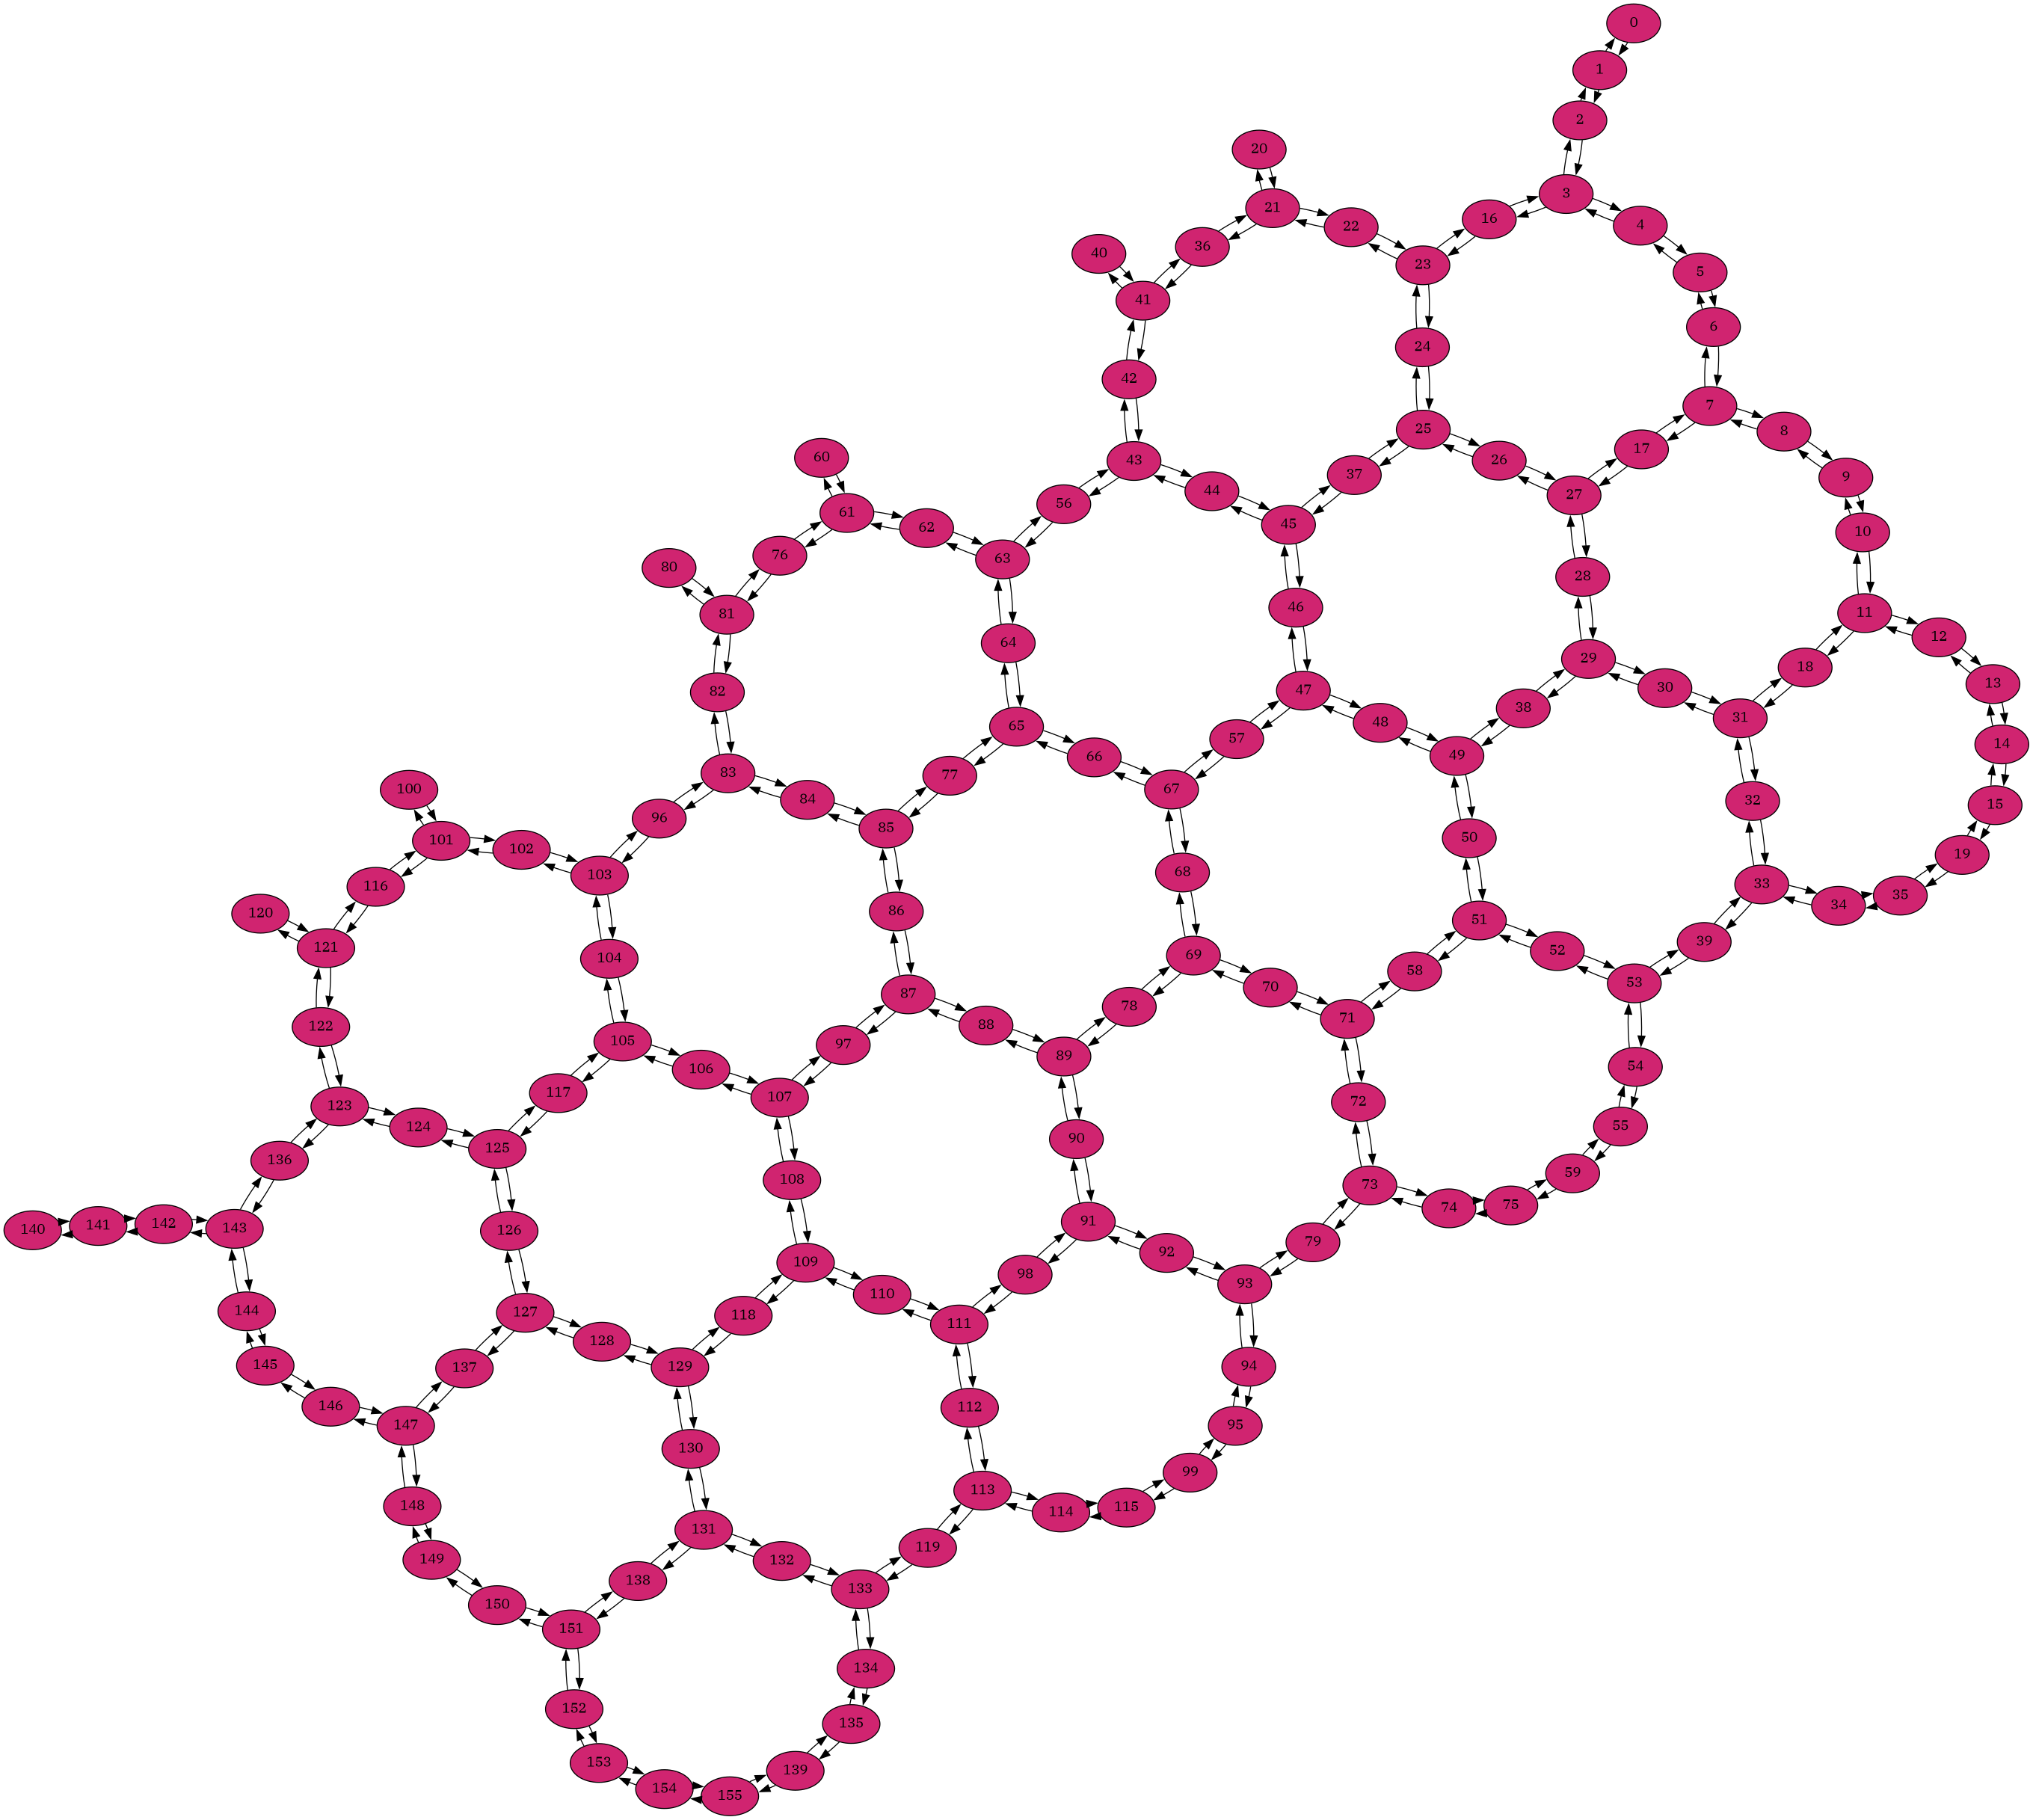
\includegraphics[valign=t, width=\textwidth]{boston}
\end{minipage}
\end{frame}

\begin{frame}[fragile]\frametitle{What makes it hard?}
\begin{itemize}\itemsep=0.8\baselineskip
\item There's no such thing as a ``copy''.
\item There's no such thing as a ``store''.
\item Each qubit can only interact with its immediate neighbours.
\end{itemize}
\pause
\medskip
\begin{block}{}
Can only shuffle ``registers'' with the xor swap trick.
\end{block}
\medskip
\begin{minted}{rust}
fn swap(a: &mut u64, b: &mut u64) {
    *a = *a ^ *b;
    *b = *a ^ *b;
    *a = *a ^ *b;
}
\end{minted}
\end{frame}

\begin{frame}\frametitle{The qubit ``routing'' problem}
\begin{itemize}\itemsep=0.8\baselineskip
\item Quantum computers are noisy; we must minimise swaps
\item We use stochastic, heuristic algorithms \ldots\ so we love threads!
\end{itemize}
\bigskip
\begin{block}{}
A \emph{lot} of our work is easily parallelised with \texttt{rayon} iterators.
\end{block}
\end{frame}

\begin{frame}[fragile]\frametitle{Micro-optimisation of core data structures}
\footnotesize
\begin{minted}{rust}
enum Op { Gate(Gate), Matrix(Box<Matrix>), Py(Box<PyOp>) }
#[repr(u8)] enum Gate { I, X, Y, Z, H, CX, RZ, /* ... */ }
\end{minted}
\pause
\smallskip
\ldots\ but\ \ \mintinline{rust}|mem::size_of::<Op>() == 16|\,!
\bigskip\bigskip
\pause
\scriptsize%
\begin{minted}{rust}
struct PackedOp(*mut ());

impl PackedOp {
   const MASK: u64 = !0b111u64;

   fn data(&self) -> *mut () {
       self.0.map_addr(|x| x & Self::MASK)
   }
   fn kind(&self) -> OpKind {
       (self.0 as u64 & !Self::MASK).into()
   }
   fn as_ref(&self) -> OpRef<'_> {
       /* ... unsafe shenaningans  ... */
   }
}   
\end{minted}
\end{frame}


\begin{frame}\frametitle{Our journey}
\begin{description}[2026]\itemsep=0.8\baselineskip
\item[2017] First release of pure-Python Qiskit
\item[2020] Qiskit swaps \texttt{NetworkX} for \texttt{rustworkx}
\item[2022] Bottleneck routines ported to Rust and \texttt{rayon}
\item[2024] Core IR data structures ported to Rust with \texttt{PyO3}
\item[2025] Exposed a C API, usable standalone or in Python extensions
\item[2026] Next-gen IRs and compiler are Rust native from day one
\end{description}
\end{frame}

\begin{frame}\frametitle{What didn't we cover?}
\begin{itemize}\itemsep=0.8\baselineskip
\item All the complex-number linear algebra (!)
\item How we use \texttt{PyO3} to expose a C API to other Python extensions
\item The whole field of quantum compilation is changing
\item Next-generation compilers mix classical and quantum
\end{itemize}
\bigskip
{\centering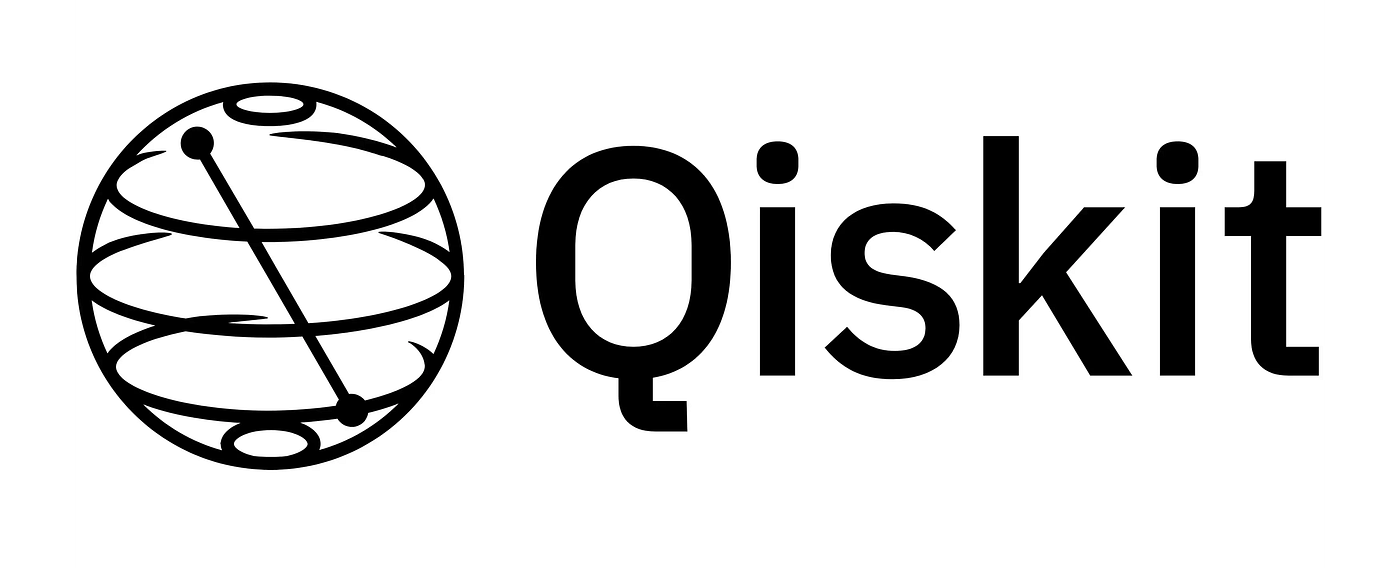
\includegraphics[width=0.3\textwidth]{qiskit-light}\par\url{https://github.com/Qiskit/qiskit}\par}
\end{frame}

\end{document}
